\subsection*{Problema 17}

\textbf{Enunciado:}
Calcular la integral indefinida:
\begin{align*}
\int \sqrt{x^2 + x + 1} \, dx
\end{align*}

\textbf{Solución:}
Para resolver la integral, primero completamos el trinomio cuadrado perfecto dentro del radical:
\begin{align*}
x^2 + x + 1 &= \left(x + \dfrac{1}{2}\right)^2 + \dfrac{3}{4}
\end{align*}

Sustituyendo esto en la integral:
\begin{align*}
I &= \int \sqrt{\left(x + \dfrac{1}{2}\right)^2 + \dfrac{3}{4}} \, dx
\end{align*}

Aplicamos la sustitución trigonométrica recomendada:
\begin{align*}
x + \dfrac{1}{2} &= \dfrac{\sqrt{3}}{2} \tan\theta \\
dx &= \dfrac{\sqrt{3}}{2} \sec^2\theta \, d\theta
\end{align*}

El término dentro de la raíz se transforma en:
\begin{align*}
\sqrt{\left(x + \dfrac{1}{2}\right)^2 + \dfrac{3}{4}} &= \sqrt{\dfrac{3}{4}\tan^2\theta + \dfrac{3}{4}} \\
&= \dfrac{\sqrt{3}}{2} \sec\theta
\end{align*}

Sustituyendo en la integral en términos de $\theta$:
\begin{align*}
I &= \int \left(\dfrac{\sqrt{3}}{2}\sec\theta\right) \left(\dfrac{\sqrt{3}}{2}\sec^2\theta \, d\theta\right) \\
&= \dfrac{3}{4} \int \sec^3\theta \, d\theta
\end{align*}

Utilizando la conocida integral de la secante cubica:
\begin{align*}
\int \sec^3\theta \, d\theta &= \dfrac{1}{2} \sec\theta \tan\theta \\
&\quad + \dfrac{1}{2} \ln|\sec\theta + \tan\theta|
\end{align*}

Regresando a la variable original $x$, recordamos que $\tan\theta = \dfrac{2x+1}{\sqrt{3}}$ y $\sec\theta = \dfrac{2\sqrt{x^2+x+1}}{\sqrt{3}}$. Sustituyendo y simplificando:
\begin{align*}
I &= \dfrac{2x+1}{4}\sqrt{x^2+x+1} \\
&\quad + \dfrac{3}{8}\ln\left|\dfrac{2\sqrt{x^2+x+1}}{\sqrt{3}} + \dfrac{2x+1}{\sqrt{3}}\right| + C
\end{align*}

\begin{figure}[H]
	\centering
	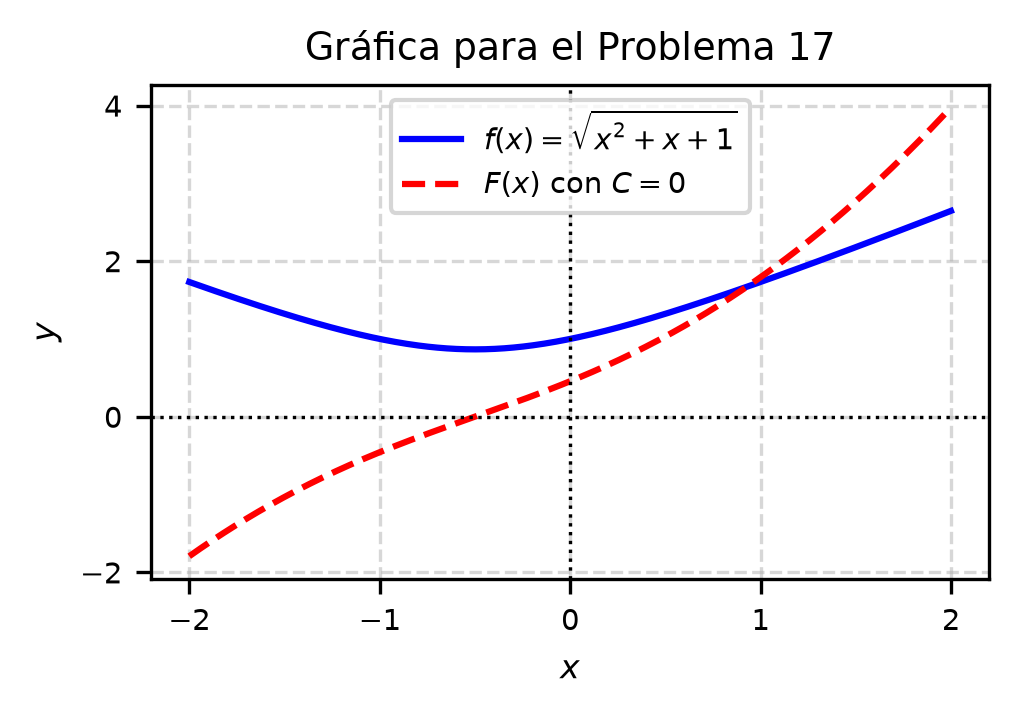
\includegraphics[width=\columnwidth]{semana_05/graficas/SEM05_P17_grafica.png}
	\caption{Representación gráfica de $f(x)$ y su antiderivada $F(x)$ evaluada para la constante de integración $C = 0$ (Problema 17).}
	\label{fig:problema17}
\end{figure}
